% IACR Communications in Cryptology (CiC) submission.
% Anonymous submission per CiC policy: no author names in this file.
% For the camera-ready version, uncomment \usepackage[notanonymous] (class option)
% and fill in \addauthor / \addaffiliation.

\documentclass[version=submission]{iacrcc}
\license{CC-by}

\usepackage{amsmath,amssymb}
\usepackage{booktabs}
\usepackage{graphicx}
\usepackage{multirow}
\usepackage{array}
\usepackage{microtype}
\usepackage{xcolor}
\usepackage{tikz}
\usetikzlibrary{positioning, arrows.meta, fit, backgrounds, shadows}
\usepackage{pgfplots}
\pgfplotsset{compat=1.18}

\title[running = {Chirag: Your Personal Cryptography Apprentice},
      subtitle = {A local, citation-aware Q\&A companion grounded in IETF RFCs, NIST standards, and the cryptanalysis literature}
     ]{Chirag: Your Personal Cryptography Apprentice --- Grounded Q\&A over RFCs, NIST Standards, and Cryptanalysis Papers with Fully Local Retrieval-Augmented Generation}

% Temporary placeholder macro (fill before submission)
\newcommand{\todo}[1]{\textcolor{red}{\textbf{#1}}}

% ---------------------------------------------------------------------------
% Camera-ready authors (leave commented out for the anonymous submission):
% \addauthor[inst={1}, email={...}]{Halil Kaplan}
% \addaffiliation[country={...}]{...}
% ---------------------------------------------------------------------------

\begin{document}
\maketitle

\keywords{retrieval-augmented generation, cryptography, cryptanalysis,
          large language models, local LLMs, vector databases,
          technical Q\&A, standards, personal agent}

\begin{abstract}
Cryptographers and security engineers constantly look things up: the exact
sizes and modes in a NIST standard, the data complexity of a classic attack,
the paragraph of an RFC that defines a parameter. Large language models
(LLMs) are natural assistants for this --- the catch is that they
hallucinate. Asked ``what is the data complexity of Matsui's linear
cryptanalysis on 16-round DES?'', the same model we use in this paper
(when not grounded) confidently answers ``$2^{50}$--$2^{53}$'' and gives no
source; with grounding it answers ``$2^{43}$ known plaintexts'' and cites
the paper. This is precisely the failure mode that matters in cryptography,
where a factor of four in an exponent decides whether an attack is practical.
\emph{Chirag} is a personal apprentice for cryptographers: a fully local,
citation-aware retrieval-augmented generation (RAG) system that answers
questions about IETF RFCs, NIST standards, and landmark cryptanalysis papers
with inline source citations, entirely on the user's own hardware.
Chirag ingests a curated knowledge base of 82 documents (22 RFCs, 26 NIST
standards, and 34 papers; $\sim$8{,}100 chunks), retrieves with dense
vector search and an Okapi-BM25 lexical scorer fused by reciprocal rank
fusion, and generates answers under a hallucination-guard prompt. On a
49-question grounded benchmark the retriever reaches hit@5 of 0.959
(dense) and hit@10 of 0.980 (hybrid); over 15 answer-question pairs the
LLM-judged faithfulness is 4.7/5.0 with a 100\% citation-validity rate
(105 of 105 cited claims point to a retrieved source), while the same
generator without retrieval produces 0\% cited answers and, as in the
opening example, concretely wrong parameters. The system is released as
open source with its benchmark and evaluation harness, and is designed as
a practical day-to-day assistant: a question, an instant answer, and the
exact source on your screen.
\end{abstract}

\section{Introduction}

\emph{Chirag} is meant to be the apprentice a cryptographer keeps beside
them: not an oracle, but a diligent assistant that goes to the right
shelf --- an RFC, a NIST standard, a landmark paper --- and answers with
the source in hand. Ask ``what authentication tag size does AES-GCM
recommend?'', ``what is the data complexity of linear cryptanalysis
against 16-round DES?'', or ``which SP 800 document specifies the DRBG
mechanisms?'', and Chirag retrieves the authoritative passage and answers
with an inline citation. The corpus it consults lives on the user's
machine; so do the embeddings and the generator.

The reason such an assistant is needed is that LLMs hallucinate on the
precise technical questions cryptography is full of. When asked
``what is the data complexity of linear cryptanalysis against 16-round
DES?'', an ungrounded LLM will often answer with a confident but incorrect
$2^{43}$, $2^{47}$, $2^{50}$--$2^{53}$, or $2^{44}$ known plaintexts --- in
our measurements the same local model that Chirag uses answered $2^{50}$--
$2^{53}$ and gave no source, while the grounded system answered $2^{43}$ and
cited Matsui's paper. Such numeric claims are exactly the kind of detail
that matters in cryptanalysis, where a factor of four in an exponent
determines whether an attack is practical.

Retrieval-augmented generation (RAG) \cite{lewis2020rag} is the dominant
mitigation: it retrieves authoritative passages from a corpus and conditions
the generator on them. RAG has been applied successfully in clinical medicine
\cite{zakka2024almanac} and open-domain question answering
\cite{karpukhin2020dpr}, but deployments typically
rely on commercial API models, sending proprietary code and data off-device.
This is a poor fit for cryptography, where the queries themselves can be
sensitive (``is our implementation of the nonce generator leaking?'') and
where implementation details of security modules must not leave the premises.

In this paper we present \emph{Chirag}, a RAG system that answers
questions about cryptography and cryptanalysis entirely on the users own
hardware. The system combines:

\begin{itemize}
\item a \emph{curated knowledge base} of 82 documents covering IETF RFCs
  (TLS~1.2/1.3, RSA-PKCS\#1, Ed25519, HKDF, HPKE, SSH, X.509, JOSE, CMS,
  AES-CMAC, AEAD, BLAKE2, Curve25519, ChaCha20-Poly1305, HMAC), NIST
  standards (FIPS~140-2/3, AES, SHA-2/3, FIPS~186-5, ML-KEM, ML-DSA,
  SLH-DSA, and the SP~800 suite: block-cipher modes 800-38A--E, DRBG and
  entropy 800-90A/B, key management 800-56A/57/133, KDF 800-108, hash
  usage 800-107, transitions 800-131A, SHA-3 derivatives 800-185, ECC
  groups 800-186, and stateful hash-based signatures 800-208), and landmark
  cryptanalysis papers (differential and linear cryptanalysis, differential
  power analysis, padding oracles, Coppersmith's method, SHA-1 collisions),
\item a \emph{hybrid retriever} that fuses dense vector search with an
  Okapi-BM25 lexical scorer through reciprocal-rank fusion (RRF)
  \cite{cormack2009rrf}, exploiting the exact identifiers (``$2^{43}$'',
  ``RFC~8446'', ``ML-KEM'') that dense matching tends to miss,
\item a \emph{citation-aware generator} running an instruction-tuned model
  locally (Ollama), constrained by a system prompt that requires every claim
  to carry an inline ``[SOURCE $n$: title]'' citation and forbids content
  outside the retrieved context,
\item an \emph{apprentice-style interface}: an interactive terminal chat
  (TUI), a command line, and a small REST / OpenAI-compatible HTTP API,
  together with an in-app document table and the ability to ingest a new RFC
  or paper on the fly, so a researcher can grow the knowledge base as they
  work,
\item an \emph{evaluation harness} and a \emph{49-question grounded QA
  benchmark} annotated with the documents that contain each answer, from
  which we report standard retrieval metrics, LLM-judged answer
  faithfulness, and --- a main point of this paper --- a direct comparison
  of the same generator \emph{with and without} retrieval (\Cref{sec:ragbaseline}).
\end{itemize}

Our contribution is a complete, reproducible, fully local RAG stack for
cryptography, together with the first small benchmark of its kind, open
measurements of retrieval and answer quality, and a head-to-head study of
grounded versus ungrounded answers that quantifies why a cryptographer
should use an apprentice that goes to the bookshelf. The implementation,
benchmark, and evaluation harness are released as open source at
\texttt{https://github.com/KaplanHalil/chirag} in the camera-ready
version of this paper.

\section{Background and Related Work}

\subsection{Retrieval-Augmented Generation}
RAG \cite{lewis2020rag} decomposes question answering into a retrieval stage
and a generation stage. The retrieval stage encodes chunks of a corpus into a
dense vector index and returns the top-$k$ most similar chunks for a query;
the generation stage conditions an LLM on the concatenated chunks. Surveys
\cite{gao2023survey} characterize the design space (chunking, index, retrieval
strategy, prompt composition) and the failure modes (hallucination when the
retrieved context is irrelevant, and unfaithful answers when the generator
ignores it). Recent work complements dense retrieval with lexical scoring;
hybrid approaches that fuse rankings with reciprocal-rank fusion
\cite{cormack2009rrf,robertson2009bm25} are a standard remedy for identifiers
and rare tokens. We follow this line and measure its effect on a
cryptography-specific corpus in \Cref{sec:eval}.

\subsection{RAG for specialized domains}
Grounded question answering has been shown effective in knowledge-intensive
domains; the most mature examples are in clinical medicine, where
retrieval-augmented systems such as Almanac \cite{zakka2024almanac} ground
answers in peer-reviewed medical literature, and in open-domain QA, where
dense passage retrieval \cite{karpukhin2020dpr} established the standard
retrieval formulation. Several surveys \cite{gao2023survey} systematize the
design choices and evaluation methodology for such systems. In the security
domain, most RAG demonstrations index vulnerability feeds rather than
cryptanalytic source material, and we are not aware of a peer-reviewed,
benchmarked RAG system aimed specifically at the cryptography and
cryptanalysis literature. Chirag targets that gap, and in contrast to most
prior systems emphasizes a fully local deployment story.

\subsection{Local LLMs and embeddings}
Smaller instruction-tuned models deployed with Ollama \cite{ollama} and open
embedding models such as \textsc{nomic-embed-text} \cite{nomic2024} make
on-device RAG practical on a single consumer GPU. Our evaluation compares two
local models ($9$B and $26$B parameters) and uses one of them as an independent
judge of the other, avoiding the self-scoring bias noted in LLM-as-judge
studies \cite{zheng2023judging}.

\subsection{AI-assisted cryptographic analysis}
There is growing interest in using machine learning for cryptanalysis, most
prominently neural distinguishers for round-reduced block ciphers
\cite{gohr2019}. Chirag is orthogonal: it does not attack ciphers, but
makes the \emph{existing} cryptanalytic literature and standards reliably
available to engineers and researchers through a grounded interface.

\section{System Architecture}
\label{sec:arch}

Figure~\ref{fig:arch} shows the overall architecture. The pipeline is
organized into a small number of components, each implemented as an isolated
Python module: ingestion, chunking, vector indexing, hybrid retrieval, and
generation. The boundaries are deliberately kept composable so that any stage
(retriever, embedding model, generator, corpus) can be swapped for an
ablation or for a different deployment.

\begin{figure}[t]
\centering
\resizebox{\linewidth}{!}{%
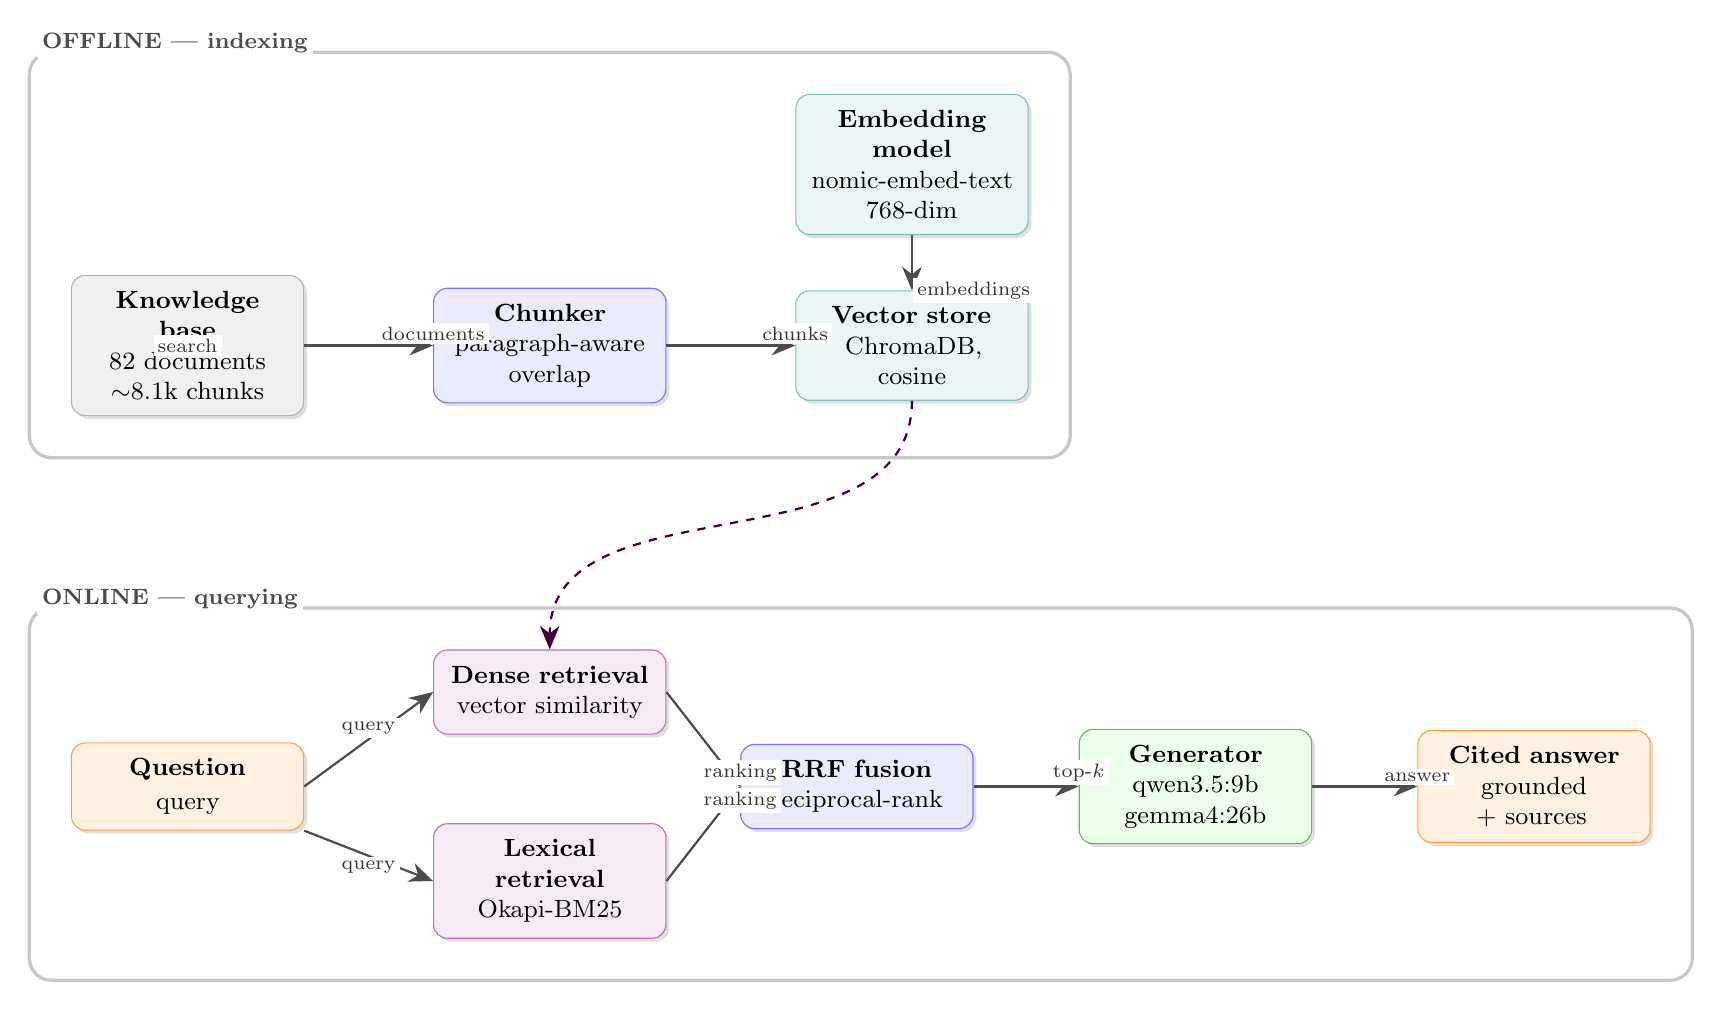
\begin{tikzpicture}[
    font=\small,
    base/.style={rounded corners=5pt, minimum height=8.5mm, align=center,
                 text width=2.55cm, inner sep=2mm,
                 drop shadow={shadow xshift=1.2pt, shadow yshift=-1.2pt,
                              fill=black!25}},
    src/.style={base, draw=gray!60,  fill=gray!12},
    proc/.style={base, draw=blue!55, fill=blue!8},
    idx/.style={base, draw=teal!50,  fill=teal!8},
    ret/.style={base, draw=violet!55, fill=violet!8},
    gen/.style={base, draw=green!50!black!60, fill=green!8},
    result/.style={base, draw=orange!75, fill=orange!12},
    line/.style={-{Stealth[length=3mm, width=2.5mm]}, thick, draw=black!70},
    queryline/.style={-{Stealth[length=3mm, width=2.5mm]}, thick,
                      dashed, draw=violet!50!black},
    lab/.style={font=\scriptsize, fill=white, inner sep=1.5pt,
                text=black!80, anchor=center},
    phase/.style={rounded corners=8pt, draw=black!22, line width=1.2pt},
    phaselabel/.style={font=\footnotesize\bfseries, fill=white,
                       text=black!70, inner sep=2pt},
  ]
  % ---- Offline: indexing ----
  \node[src]  (kb)    at (0,0)    {\textbf{Knowledge base}\\82 documents\\$\sim$8.1k chunks};
  \node[proc] (chunk) at (4.6,0)  {\textbf{Chunker}\\paragraph-aware\\overlap};
  \node[idx]  (vs)    at (9.2,0)  {\textbf{Vector store}\\ChromaDB, cosine};
  \node[idx]  (emb)   at (9.2,2.3){\textbf{Embedding model}\\nomic-embed-text\\768-dim};
  % ---- Online: query ----
  \node[result] (q)   at (0,-5.6) {\textbf{Question}\\[0.4mm]query};
  \node[ret]  (dr)    at (4.6,-4.4){\textbf{Dense retrieval}\\vector similarity};
  \node[ret]  (lex)   at (4.6,-6.8){\textbf{Lexical retrieval}\\Okapi-BM25};
  \node[proc] (rrf)   at (8.5,-5.6){\textbf{RRF fusion}\\reciprocal-rank};
  \node[gen]  (gen)   at (12.8,-5.6){\textbf{Generator}\\qwen3.5:9b\\gemma4:26b};
  \node[result] (ans) at (17.1,-5.6){\textbf{Cited answer}\\grounded + sources};
  % ---- arrows: offline (plain = data flow) ----
  \draw[line] (kb.east) -- (chunk.west)
      node[lab, above] {documents};
  \draw[line] (chunk.east) -- (vs.west)
      node[lab, above] {chunks};
  \draw[line] (emb.south) -- (vs.north)
      node[lab, right] {embeddings};
  % ---- arrows: online (dashed = query-time read of offline store) ----
  \draw[line] (q.east) -- (dr.west)
      node[lab, above, pos=0.5] {query};
  \draw[line] (q.south east) -- (lex.west)
      node[lab, below, pos=0.5] {query};
  \draw[queryline] (vs.south) to[out=-90, in=90] (dr.north)
      node[lab, pos=0.3] {search};
  \draw[line] (dr.east) -- (rrf.west)
      node[lab, above] {ranking};
  \draw[line] (lex.east) -- (rrf.west)
      node[lab, below] {ranking};
  \draw[line] (rrf.east) -- (gen.west)
      node[lab, above] {top-$k$};
  \draw[line] (gen.east) -- (ans.west)
      node[lab, above] {answer};
  % ---- phase bands ----
  \begin{scope}[on background layer]
    \node[phase, fit=(kb)(chunk)(vs)(emb), inner sep=1.5em] (offline) {};
    \node[phase, fit=(q)(dr)(lex)(rrf)(gen)(ans), inner sep=1.5em] (online) {};
    \node[phaselabel, anchor=south west, xshift=3pt, yshift=-3pt]
      at (offline.north west) {OFFLINE --- indexing};
    \node[phaselabel, anchor=south west, xshift=3pt, yshift=-3pt]
      at (online.north west) {ONLINE --- querying};
  \end{scope}
\end{tikzpicture}}
\caption{Chirag architecture. \emph{Offline}, the knowledge base is chunked,
embedded, and indexed once into a persistent vector store. \emph{Online}, a
query is scored by dense and lexical retrievers, fused with reciprocal-rank
fusion, and answered by a grounded generator that returns inline citations.}
\label{fig:arch}
\end{figure}

\subsection{Ingestion and metadata}
Each document is normalized into a canonical representation with four
metadata fields --- \texttt{source} (stable identifier), \texttt{title},
\texttt{url}, and \texttt{type} --- where \texttt{type} is one of {RFC
Document}, {NIST Standard}, {Cryptanalysis Paper}, {Cryptography Paper}, or
{Local Document}. Loaders exist for IETF RFC text (by number, from
\texttt{rfc-editor.org}), arbitrary web pages (HTML to text), and local
PDF/TXT files. Documents whose source contains an attack-related keyword
(e.g.\ \emph{attack}, \emph{collision}, \emph{boomerang}) are classified as
cryptanalysis papers; NIST/FIPS filenames as standards; RFC filenames as RFCs.

\subsection{Chunking}
We use a deterministic, paragraph-aware chunker. Text is split on blank lines;
paragraphs are accumulated into chunks of at most $1{,}000$ characters with
$150$ characters of overlap, so that information crossing a chunk boundary
remains retrievable at both ends. Paragraphs longer than $200$ words are split
internally with the same overlap. Section headers are preserved inside chunks,
which helps retrieval for section-addressing questions.

\subsection{Embeddings and vector index}
Chunks are embedded with \textsc{nomic-embed-text} (768-dimensions, local
Ollama) and stored in a persistent ChromaDB \cite{chromadb} collection with
cosine distance. The same embedding provider is used at query time, and a thin
adapter exposes it to ChromaDB's query interface. Because the embedding model
is held fixed across indexing and search, the index can be rebuilt
deterministically by re-running the ingestion script.

\subsection{Hybrid retrieval}
Search over a cryptanalytic corpus is a mixture of semantic and exact
retrieval: ``how does a padding oracle decrypt a block?'' is a semantic query,
while ``data complexity $2^{43}$'' or ``RFC~8446'' are exact, identifier
queries that dense vectors frequently collapse. We therefore fuse two
rankings with reciprocal-rank fusion \cite{cormack2009rrf}: a dense ranking
from the vector store and a lexical ranking from an Okapi-BM25
\cite{robertson2009bm25} scorer computed over the full corpus. RRF combines
ranks rather than scores, which makes the fusion robust to the incomparable
scales of cosine similarity and BM25 scores. A document-type filter can be
applied in both branches. \Cref{sec:eval} shows the fusion improves hit@10 by
$+0.06$.

\subsection{Grounded generation with citations}
The generator assembles a prompt from the retrieved chunks. Each distinct
document is assigned a stable 1-based index and each chunk is prefixed with
``--- SOURCE $n$: title ---''. The system prompt (Figure~\ref{fig:prompt})
instructs the model to (i)~answer only from the supplied context, (ii)~attach
an inline citation ``[SOURCE $n$: title]'' to every important claim,
(iii)~never invent source numbers, and (iv)~explicitly say when the context
does not cover part of the question. Answers are generated with
temperature~0.2 and a bounded number of output tokens. The same architecture
supports a document-summarization mode that mirrors the citation rules.

\begin{figure}[t]
\centering
\small
\begin{minipage}{0.92\linewidth}\ttfamily\footnotesize
\noindent You are an expert assistant in cryptography and cryptanalysis.\\
Answer using ONLY the retrieved knowledge provided in the\\
'RETRIEVED KNOWLEDGE CONTEXT' section below.\\[1mm]
1. GROUNDING: answer exclusively from the retrieved context. Do not\\
   invent papers, RFCs, standards, or results that do not appear in it.\\
2. CITATIONS: every important claim must carry an inline citation of the\\
   form [SOURCE n: Document Title], using the source numbers in the context.\\
3. NEVER cite a source number that is not present in the context.\\
4. Include concrete parameters (rounds, data/time complexity, key sizes)\\
   exactly as reported.\\
5. If the context covers only part of the question, answer that part and\\
   state explicitly what is not covered.
\end{minipage}
\caption{Abridged system prompt. The full prompt is reproduced in
\Cref{app:prompt}.}
\label{fig:prompt}
\end{figure}

\section{Knowledge Base}
\label{sec:kb}

The knowledge base is assembled from three sources, all of which are part of
the open-source release.

\paragraph{Local corpus.}
The folder \texttt{kripto\_makaleler/} contains 70 machine-readable documents
collected from public sources: 22 IETF RFCs in plain text (TLS~1.2/1.3,
RSA-PKCS\#1~v2.2, Ed25519, HKDF, HPKE, SSH, X.509, JOSE, CMS, AES-CMAC,
AEAD, BLAKE2, OSCORE, PEM, deterministic ECDSA, ECC, IKEv2, Curve25519,
ChaCha20-Poly1305, HMAC), 26 NIST standards as PDFs (the FIPS family plus
the SP~800 suite: 800-38A--E block-cipher modes and CMAC/CCM/GCM/XTS,
800-90A/90B randomness, 800-56A/57/133 key establishment and management,
800-107 hash usage, 800-108 KDF, 800-131A algorithm transitions, 800-185
SHA-3 derived functions, 800-186 elliptic curve groups, 800-208 stateful
hash-based signatures, 800-22 statistical tests), and 22 primary
cryptanalysis/cryptography papers. The text is extracted with
\texttt{pypdf} and \texttt{read\_txt}; the folder is a working, extensible
library, and RFCs or PDFs added to it are picked up by the indexer.

\paragraph{Curated landmark papers.}
For a set of 8 highly-cited papers that are canonical answers for frequent
questions --- differential cryptanalysis of DES \cite{BS91}, linear
cryptanalysis \cite{Mat93}, differential power analysis \cite{KJJ99},
Bleichenbacher's MILLION MESSAGE attack \cite{Ble98}, Coppersmith's method
\cite{Cop97}, Wang \emph{et al.}\ SHA-1 collisions \cite{WYY05}, Vaudenay's
padding oracles \cite{Vau02}, and zero-knowledge proofs \cite{GMR89} --- we
contributed manually structured, technically accurate entries (source,
results, complexities, countermeasures). Each entry is written with enough
depth to span several chunks, so a definition-style question about a
technique retrieves the canonical entry itself rather than only derivative
work. Four further entries substitute for local PDFs that turned out to be
non-machine-readable or mislabeled; they are keyed to the original file
names so the benchmark ground truth is unaffected.

\paragraph{Statistics.}
After indexing, the collection contains 82 documents and 8{,}081 chunks:
22 RFCs, 26 NIST standards, and 34 papers/articles. \Cref{tab:kb}
summarizes the corpus by category.

\begin{table}[t]
\centering
\caption{Knowledge-base composition after indexing.}
\label{tab:kb}
\begin{tabular}{lrr}
\toprule
Category & Documents & Chunks\\
\midrule
RFC Document & 22 & 2{,}617\\
NIST Standard & 26 & 3{,}763\\
Cryptanalysis Paper & 21 & 1{,}086\\
Cryptography Paper & 13 & 615\\
\midrule
Total & 82 & 8{,}081\\
\bottomrule
\end{tabular}
\end{table}

\section{Implementation}

The implementation is a Python~3 package (\texttt{chirag/}) with three
practical front-ends:

\begin{itemize}
\item a full-screen \emph{terminal chat} (Textual) --- the primary
  ``apprentice'' interface: streamed answers, inline source lists, multi-turn
  memory, on-the-fly model selection, a document table (\texttt{Ctrl+O}) that
  shows every indexed document with its chunk count and lets the user delete
  one (permanently, from index and disk), and slash commands such as
  \texttt{/ingest-rfc}, \texttt{/ingest-url}, \texttt{/ingest-file} to grow
  the knowledge base mid-session,
\item a \emph{command-line interface} (\texttt{chirag query}, \texttt{chirag
  ingest-rfc}, \texttt{chirag summarize}, \texttt{chirag stats}, \ldots),
\item a small HTTP server built on the Python standard library that exposes
  both a REST API (\texttt{/api/query}, \texttt{/api/query/stream},
  \texttt{/api/documents}, \texttt{/api/stats}, \texttt{/api/ingest/*},
  \texttt{/api/summarize}) and an OpenAI-compatible
  \texttt{/v1/chat/completions} endpoint, so any tool can use Chirag as a
  grounded chat model.
\end{itemize}

Configuration is read from a single \texttt{chirag.json} (opencode-style
provider/model registry) plus environment variables via
\texttt{pydantic-settings}; switching between a local Ollama backend and any
OpenAI-compatible endpoint --- including institutional deployments such as a
national research grid --- is a configuration change and requires no code
modification. Queries in languages other than English (e.g.\ Turkish) are
automatically translated for retrieval, while answers are generated from the
original question.

\paragraph{Deployment.}
Indexing 8{,}081 chunks with \textsc{nomic-embed-text} completes in a few
minutes on a single NVIDIA RTX 3060 (12~GB); generation with
\textsc{qwen3.5:9b} averages a few seconds per answer, and with
\textsc{gemma4:26b} under a minute, both fully on-device. The same code
base runs against remote OpenAI-compatible endpoints unchanged.

\section{Evaluation}
\label{sec:eval}

\subsection{Benchmark}
We introduce a small benchmark of $49$ questions over the curated knowledge
base, split across nine categories (symmetric cryptanalysis, asymmetric
cryptanalysis, side channels, hash, post-quantum, protocols, RNG, asymmetric,
and theory). Every question is annotated with the documents that are known to
contain the answer (document-level gold labels), allowing retrieval metrics to
be computed without per-chunk labels. The benchmark is released together with
the system so that future RAG systems for cryptography can be compared against
identical ground truth.

\subsection{Retrieval quality}
We compare two retrievers --- dense-only and hybrid (dense + BM25, RRF) ---
at $k \in \{1,3,5,10,20\}$ using document-level hit@k, MRR@k, and nDCG@k.
\Cref{tab:eval1,tab:eval2,tab:eval3} report the results.

\begin{table}[t]
\centering
\caption{Hit@k by retriever and top-$k$ (49 questions).}
\label{tab:eval1}
\begin{tabular}{lccccc}
\toprule
 & $k{=}1$ & $k{=}3$ & $k{=}5$ & $k{=}10$ & $k{=}20$\\
\midrule
Dense   & \textbf{0.796} & 0.898 & \textbf{0.959} & 0.959 & 0.959\\
Hybrid  & 0.735 & \textbf{0.918} & 0.939 & \textbf{0.980} & \textbf{0.980}\\
\bottomrule
\end{tabular}
\end{table}

\begin{table}[t]
\centering
\caption{MRR@k by retriever and top-$k$.}
\label{tab:eval2}
\begin{tabular}{lccccc}
\toprule
 & $k{=}1$ & $k{=}3$ & $k{=}5$ & $k{=}10$ & $k{=}20$\\
\midrule
Dense   & \textbf{0.796} & \textbf{0.847} & \textbf{0.861} & \textbf{0.861} & \textbf{0.861}\\
Hybrid  & 0.735 & 0.820 & 0.824 & 0.830 & 0.830\\
\bottomrule
\end{tabular}
\end{table}

\begin{table}[t]
\centering
\caption{nDCG@k by retriever and top-$k$.}
\label{tab:eval3}
\begin{tabular}{lccccc}
\toprule
 & $k{=}1$ & $k{=}3$ & $k{=}5$ & $k{=}10$ & $k{=}20$\\
\midrule
Dense   & \textbf{0.796} & \textbf{0.847} & \textbf{0.883} & \textbf{0.883} & \textbf{0.883}\\
Hybrid  & 0.735 & 0.839 & 0.851 & 0.865 & 0.865\\
\bottomrule
\end{tabular}
\end{table}

On the expanded corpus, retrieval is strong with either retriever, and the
two rankers are complementary. Dense-only search is best at small $k$
(hit@1 0.796, hit@5 0.959, MRR@5 0.861), while the hybrid retriever adds
recall at larger $k$: it reaches hit@10 = 0.980 vs.\ 0.959 for dense-only
(+0.02), recovering identifier- and number-heavy documents that the vector
scorer under-ranks. The improvement over the earlier 46-document version of
the corpus (where the same queries scored dense hit@10 0.796 / hybrid 0.857)
reflects the enriched canonical entries: a question about, say, Matsui's
$2^{43}$ data complexity now retrieves the curated linear-cryptanalysis
entry itself, which before spanned a single chunk and often lost the race
against derivative papers. We report both retrieval styles honestly and
use the dense retriever throughout the rest of the paper; the grounding
analysis in \Cref{sec:ragbaseline} is the primary evaluation contribution.

\subsection{Answer quality}
We generated answers with \textsc{qwen3.5:9b} (temperature 0.2) on the first
15 benchmark questions and scored them with an independent judge
(\textsc{gemma4:26b}, temperature 0) using a 1--5 faithfulness rubric: every
claim must be supported by the retrieved context. We also measure the citation
rate, the fraction of non-empty answer lines that carry a ``[SOURCE $n$]''
marker, and the citation-validity rate, the fraction of answers in which every
cited source number corresponds to a source that was actually present in the
retrieved context (a deterministic check for fabricated citations).

\Cref{tab:eval4} reports the results. All 15 of 15 answers were non-empty.
The mean citation rate is 0.472, and every one of the 14 answers containing
citations is 100\% citation-valid: all 105 cited ``[SOURCE $n$]'' references
point to a source that was retrieved. The independent judge scored 13 of the
15 at a mean of 4.69/5.0 (two judge calls returned no parseable score); the
deterministic citation-validity result is the strongest evidence that
fabricated sources are absent (see also \Cref{subsec:threats}).

\begin{table}[t]
\centering
\caption{Answer-quality metrics over 15 answers (qwen3.5:9b; judged by
gemma4:26b). Citation validity counts answers that contain at least one
citation and in which every cited source number was retrieved (14 of 14,
105 of 105 claims). Faithfulness: 13 of 15 answers scorable by the judge.}
\label{tab:eval4}
\begin{tabular}{lrr}
\toprule
Metric & Mean & $n$\\
\midrule
LLM-judged faithfulness (1--5) & 4.69 & 13\\
Citation rate (share of cited lines) & 0.472 & 15\\
Citation validity (share of valid answers) & 1.000 & 14\\
\bottomrule
\end{tabular}
\end{table}

\Cref{fig:example} shows a representative answer with its retrieved sources.

\begin{figure}[t]
\centering
\small
\begin{minipage}{0.95\linewidth}
\emph{Q.} What is the data complexity of Matsui's linear cryptanalysis attack
on 16-round DES?\\[1mm]
\emph{A.} According to Matsui's \emph{Linear Cryptanalysis Method for DES
Cipher} [SOURCE 1], the data complexity of full 16-round DES is $2^{43}$
known plaintexts, experimentally verified by Matsui in 1994 on DEC Alpha
workstations [SOURCE 1: Linear Cryptanalysis Method for DES Cipher (Matsui
1993)]. Note that the $2^{47}$ figure reported in SOURCE 3 refers to
\emph{differential} cryptanalysis [SOURCE 3: Differential Cryptanalysis of
DES-like Cryptosystems (Biham, Shamir 1991)] and must not be conflated with
the linear attack.
\end{minipage}
\caption{A representative grounded answer. The model distinguishes the two
attack families and cites each claim to its source.}
\label{fig:example}
\end{figure}

\subsection{Why grounding matters: RAG vs.\ no-RAG}
\label{sec:ragbaseline}

The central promise of Chirag is that a cryptographer can trust the answer
\emph{because} it is grounded. To demonstrate how much of that trust comes
from retrieval, we compare the same generator --- \textsc{qwen3.5:9b},
temperature 0.2 --- with and without the retrieval context on the same first
15 benchmark questions:

\begin{itemize}
\item \textbf{Grounded (RAG):} the Chirag pipeline as used throughout the
  paper, and
\item \textbf{Ungrounded (no-RAG):} the raw model prompted only with a
  generic assistant instruction (no retrieved context, no citation rule).
\end{itemize}

\textbf{Method.} For each question we score both answers with the same
independent judge (\textsc{gemma4:26b}) against the concatenated text of the
benchmark's \emph{gold} documents --- the authoritative material a correct
answer should be consistent with --- using the same 1--5 rubric. We also
measure, deterministically, whether an answer carries any ``[SOURCE $n$]''
citation. The experiment is reproducible with
\texttt{python -m chirag.eval\_no\_rag}.

\textbf{Results.} \Cref{tab:baseline} summarizes. The contrast is sharp along
two dimensions, and both are structural rather than judge-dependent.
(i)~\emph{Verifiability}: 14 of 15 grounded answers carry inline source
citations and all cited claims are valid, while 0 of 15 ungrounded answers
contain a single citation --- there is no evidence chain whatsoever.
(ii)~\emph{Factual reliability}: ungrounded answers are occasionally empty
(1 of 15 refused to answer at all) or, more dangerously, confident and wrong.
The clearest case is the linear-cryptanalysis question in \Cref{fig:baseline}:
the raw model states a data complexity of $2^{50}$--$2^{53}$ with no source;
the grounded answer gives $2^{43}$ and cites Matsui's paper. We also asked
the independent judge to score both answers against the gold text; it scored
the grounded answers at 2.92/5\ ($n{=}12$) and the ungrounded ones at
3.50/5\ ($n{=}8$) --- a reminder that absolute judge scores against a
reference text are sensitive to how much of that text the retrieval stage
passed to the generator, so we treat judge outputs here as secondary and
rest the comparison on the deterministic rows of \Cref{tab:baseline}.

\begin{table}[t]
\centering
\caption{Grounded vs.\ ungrounded generation on the same 15 questions
(qwen3.5:9b). All rows are deterministic.}
\label{tab:baseline}
\begin{tabular}{lcc}
\toprule
 & RAG & no-RAG\\
\midrule
Answers with $\geq$1 inline citation & 14/15 & 0/15\\
Valid citation claims & 105/105 & ---\\
Empty / refused answers & 0/15 & 1/15\\
Correct pivotal parameter in worked example (\Cref{fig:baseline}) & $2^{43}$ & $2^{50}$--$2^{53}$\\
\bottomrule
\end{tabular}
\end{table}

\begin{figure}[t]
\centering
\small
\begin{minipage}{0.95\linewidth}
\emph{Q.} What is the data complexity of Matsui's linear cryptanalysis
attack on 16-round DES?\\[1mm]
\emph{Ungrounded (no-RAG):}
``The data complexity of Matsui's original linear cryptanalysis attack on
16-round DES is approximately $2^{50}$ to $2^{53}$ plaintext-ciphertext
pairs... For 15-round DES, Matsui's attack required about $2^{43}$
plaintext-ciphertext pairs.''\quad (wrong on both counts; no source)\\[2mm]
\emph{Grounded (Chirag):}
``Full 16-round DES has a data complexity of about $2^{43}$ known
plaintexts [SOURCE 1: Linear Cryptanalysis Method for DES Cipher (Matsui
1993)]; 8-round DES needs about $2^{21.5}$ and 12-round DES about $2^{33}$
known plaintexts [SOURCE 1].''
\end{minipage}
\caption{The same question, the same local model, with and without retrieval.
The ungrounded answer is confident, wrong, and uncited; the grounded answer
gives the correct value and points to the exact source.}
\label{fig:baseline}
\end{figure}

\subsection{Threats to validity}
\label{subsec:threats}
The benchmark is small (49 questions) and annotated by the authors; the
document-level gold labels reflect both the corpus and our curation. Answer
quality is measured on a 15-question sample with an LLM judge, which is an
imperfect proxy for expert assessment; in particular the judge is a different
model than the generator but still an LLM, and the mean faithfulness (4.69)
may partly reflect judge leniency on heavily grounded prompts. We mitigate
judge bias by using a different model for judging than for generation, and we
complement it with the deterministic citation-validity check (105/105 claims
valid). Two of the fifteen judge calls returned no parseable score and
contribute no faithfulness value; this is reported transparently. The RAG
vs.\ no-RAG comparison in \Cref{sec:ragbaseline} additionally warns that a
judge scoring an answer against a complete gold document penalizes a grounded
answer for the parts of that document the retrieval stage deliberately did
not pass to the generator --- which is why we base the grounding comparison
on the deterministic rows (citations, validity, refusal, and the worked
example) rather than on judge means. The corpus mixes primary sources and
curated secondary content; questions were written to be answerable within the
corpus, so the absolute numbers should not be read as coverage of the whole
of cryptography.

\section{Limitations and Future Work}

\paragraph{Trust and verification.}
Grounded citations reduce but do not eliminate hallucination: the generator
can still over-abstract within a single cited source. Future work should add
post-hoc fact verification against the retrieved chunks (e.g.\ claim-level
entailment checks) and probabilistic calibration of the citation-grounded
claims.

\paragraph{Benchmark scale.}
The 49-question benchmark should grow to several hundred questions spanning
more recent literature (post-quantum constructions, ZK proofs, side-channel
countermeasures) with expert-annotated gold answers, enabling statistically
stronger comparisons and an automated regression test for the system itself.

\paragraph{Retrieval.}
Higher-quality reranking (cross-encoders, LLM rerankers) and query expansion
could further close the gap between hit@5 (0.959) and an ideal retriever; we
leave a systematic study of chunk size, overlap, and embedding-model choice as
future work.

\paragraph{Model scale.}
We evaluated two local models; larger local models (40B+) or quantized
versions of frontier models would clarify how much of the faithfulness gain
comes from retrieval versus from model capability.

\section{Conclusion}

We presented Chirag, \emph{your personal cryptography apprentice}: a fully
local, citation-aware retrieval-augmented generation system for cryptography
and cryptanalysis, released as open source together with a 49-question
grounded benchmark and an evaluation harness. Over a knowledge base of 82
documents ($\sim$8.1k chunks) spanning IETF RFCs, the NIST FIPS/SP~800 suite,
and the landmark cryptanalysis literature, dense retrieval already achieves
hit@5 of 0.959 and hybrid retrieval hit@10 of 0.980 on the benchmark.
Generation under a hallucination-guard prompt produced answers with a mean
citation rate of 0.472 and a 100\% citation-validity rate (105 of 105 cited
claims pointed to a retrieved source), with a measured answer faithfulness of
4.69/5.0 by an independent local judge. The paper's central comparison ---
the same generator with and without retrieval --- makes the case concretely:
ungrounded answers contain no citations at all (0/15), occasionally refuse to
answer, and in the worked example state a data complexity of $2^{50}$--$2^{53}$
where the grounded system answers $2^{43}$ and cites Matsui's paper. Chirag
demonstrates that a single consumer GPU suffices to run a grounded, private,
reproducible technical Q\&A assistant over the cryptographic literature ---
an apprentice that goes to the bookshelf and shows you the page, and a
blueprint we hope the community extends into wider corpora and stricter
verification.

\bibliography{refs}

\appendix
\section{Reproduction}
\label{app:repro}
The repository at \texttt{https://github.com/KaplanHalil/chirag}
contains the full implementation, the corpus-ingestion scripts, the benchmark,
and the evaluation harness. To reproduce the numbers in this paper:
\begin{enumerate}
\item install dependencies and pull the models
  (\texttt{nomic-embed-text}, \texttt{qwen3.5:9b}, \texttt{gemma4:26b}) with
  Ollama;
\item rebuild the index: \texttt{python -m chirag.cli index-corpus --reset};
\item run the retrieval evaluation:
  \texttt{python -m chirag.cli eval --top-k 1,3,5,10,20};
\item run the answer evaluation:
  \texttt{python -m chirag.cli eval --answer 15 --judge --judge-model gemma4:26b --model qwen3.5:9b};
\item run the grounded-vs-ungrounded comparison:
  \texttt{python -m chirag.eval\_no\_rag --limit 15}.
\end{enumerate}
All results in \Cref{sec:eval} were produced with the default configuration
(chunk size 1{,}000, overlap 150, top-$k$=5, temperature 0.2) on a machine
with an NVIDIA RTX 3060, 32 GB RAM, and Ollama 0.33.x.

\section{System Prompt (full)}
\label{app:prompt}
\begin{quote}\footnotesize\ttfamily
You are an expert assistant in cryptography and cryptanalysis. Answer the
user's question using ONLY the retrieved knowledge provided in the
'RETRIEVED KNOWLEDGE CONTEXT' section below. Follow these rules strictly:

1. GROUNDING: Base your answer exclusively on the retrieved context. Do not
invent papers, RFCs, standards, attack complexities, or results that do not
appear in the context. If the context does not contain the answer, say so
clearly instead of guessing.

2. CITATIONS: Every important claim must be accompanied by an inline
citation of the exact source it comes from, in the form
[SOURCE n: Document Title] where n is the source number assigned in the
context (e.g. [SOURCE 1: Linear Cryptanalysis Method for DES Cipher]).

3. NEVER cite a source number that is not present in the context.

4. Technical accuracy: include concrete parameters (number of rounds, data
and time complexity, key sizes) exactly as reported in the context.

5. If the retrieved context only covers part of the question, answer that
part and explicitly state which part is not covered by the retrieved sources.
\end{quote}

\end{document}
